\chapter{Test}

\section{Redux DevTools}
I browser più famosi mettono a disposizione un'estesione per il controllo degli stati di Redux in tempo reale.
Redux DevTools è l'estensione utilizzata per il debug e i test degli stati.\newline
In realtà è possibile utilizzare Redux DevTools con qualsiasi altra architettura che utilizza gli stati.
\begin{figure}[H]
    \caption{Finestra di Redux Devtool}
    \centering
    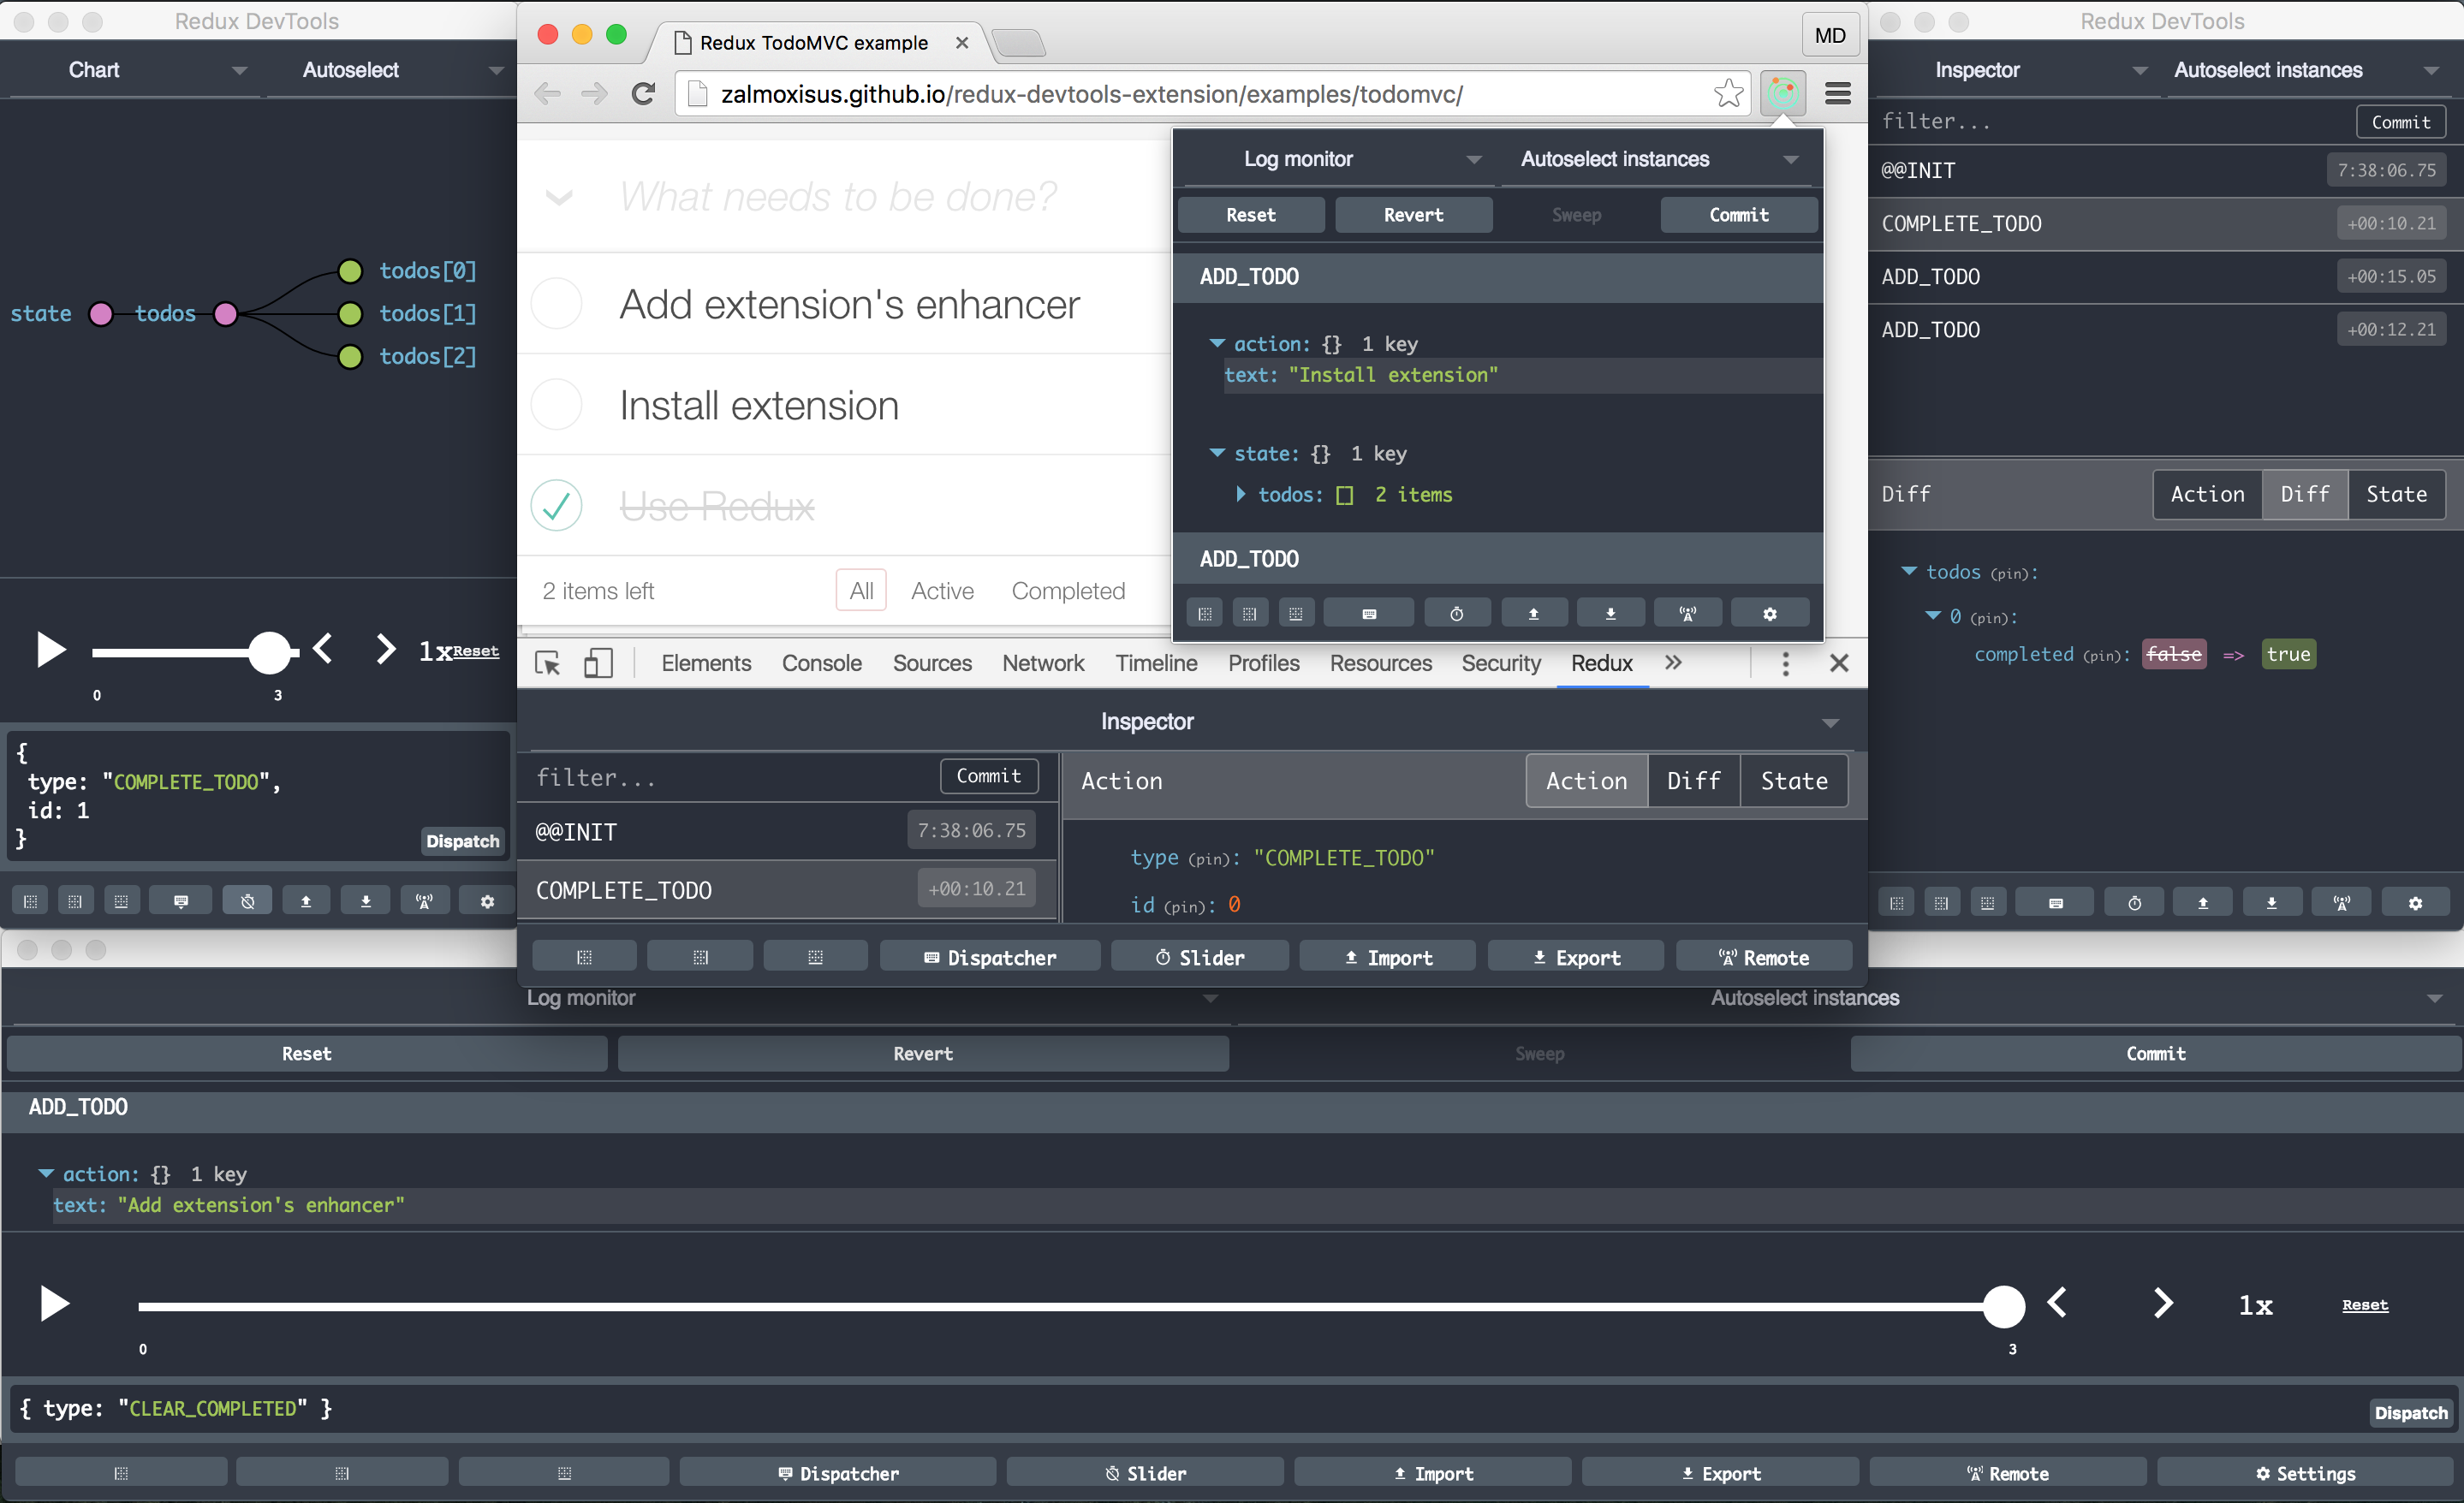
\includegraphics[width=150mm]{img/test/redux_screen.png}
    \label{fig:reduxDevWindow}
\end{figure}

\noindent Redux DevTools è stato utilizzato soprattutto per testare il corretto funzionamento di comunicazione tramite WebSocket. 
\begin{figure}[H]
    \caption{Logo di Redux DevTools}
    \centering
    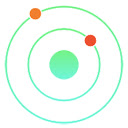
\includegraphics[width=30mm]{img/logos/redux_devtool.jpg}
    \label{fig:reduxDev}
\end{figure}

\section{Axe DevTools}
Il set di tool di cui ci siamo serviti per monitorare ed eventualmente correggere questioni riguardanti l'accessibilità nel presente applicativo. Axe DevTools è un insieme di strumenti leader del settore, che permette tramite un'estensione installabile direttamente su browser di ispezionare una pagina web o sottoparti di essa allo scopo di individuare problemi di accessibilità. Il tool poi procede con il suddividere i problemi in varie categorie a seconda della gravità dei problemi eventualmente riscontrati:


\begin{itemize}
    \item \textbf{critical}: il set di errori più gravi che potrebbero compromettere la navigabilità del sito;
    \item \textbf{serious}: set di errori che non compromettono la navigabilità ma possono ostacolare o peggiorare l'esperienza dell'utente all'interno di un sito;
    \item \textbf{moderate}: errori che principalmente riguardano il mancato utilizzo di pratiche ritenute opportune, tuttavia non fondamentali per garantire l'accessibilità;
    \item \textbf{minor}:  dove sono evidenziate sviste ed errori che impattano in maniera inferiore sull'esperienza utente.
\end{itemize}

Oltre a questa comoda suddivisione i tool permettono anche di ragguppare più errore dello stesso tipo che avrebbero soluzione comune, solitamente predispongono una descrizione del problema identificato e delle linee guida per risolverlo.

\begin{figure}[H]
    \caption{Logo di Axe DevTools}
    \centering
    
\includegraphics[width=80mm]{img/logos/axeDevtools_logo.png}
    \label{fig:axeDevtools}
\end{figure}

\section{Postman}

L'app Postman è un comodo strumento per testare una API REST in API Gateway. Postman è stato utilizzato per effettuare testing sulle API del server.\newline
Grazie a Postman è possibile creare richieste verso una certa API e verificare il contenuto e il formato delle risposte.\newline
Ogni API del sistema è stata testata, creando richieste opportune per verificare che tutto andasse a buon fine, e richieste sbagliate o non valide per verificare che il sistema rispondesse in maniera comunque consona e giusta.
\begin{figure}[H]
    \caption{Schermata della Workspace Postman di GuessR }
    \centering
    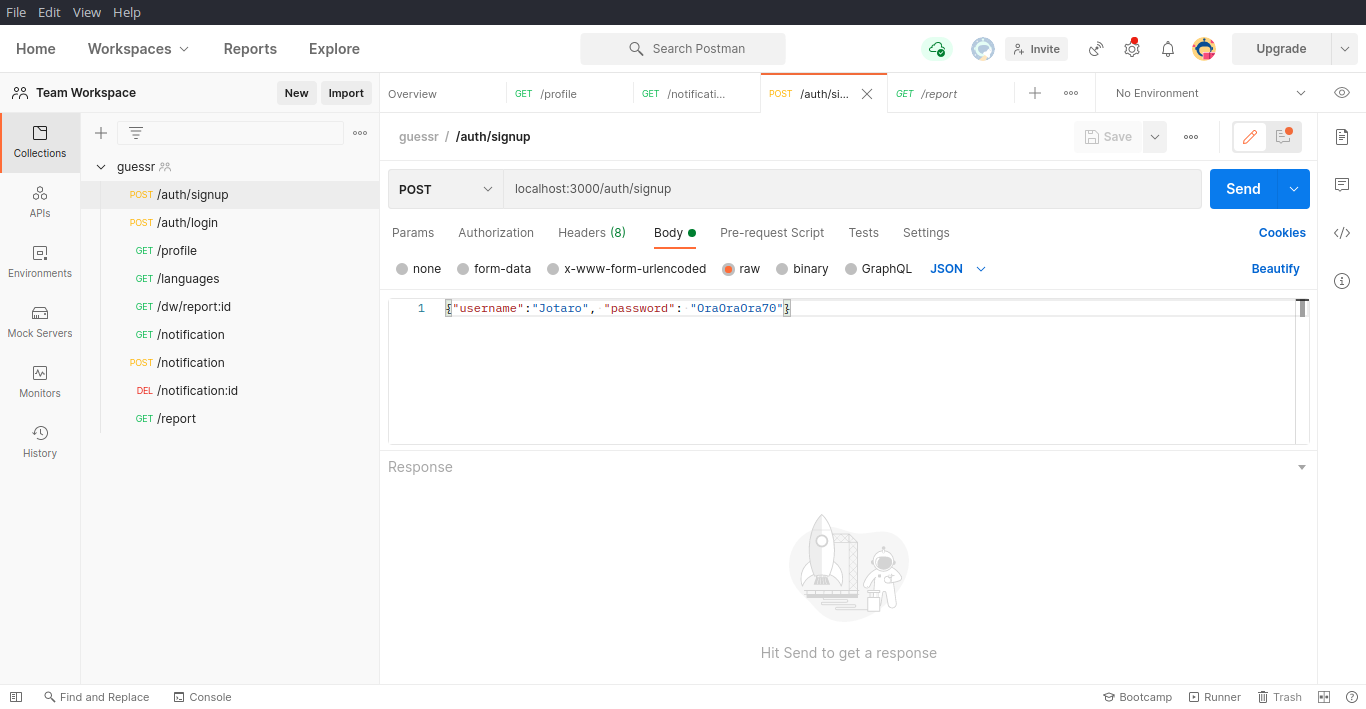
\includegraphics[width=160mm]{img/test/postman.png}
    \label{fig:postmanScreem}
\end{figure}
Per chiamare un'API utilizzando Postman è necessario:
\begin{itemize}
    \item Immettere l'URL dell'endpoint di una richiesta nella barra degli indirizzi (nel nostro caso il server) e selezionare il metodo HTTP appropriato nell'elenco a discesa a sinistra della barra degli indirizzi.
    \item Se necessario, scegliere la scheda Authorization (Autorizzazione). Per le route protette dal middleware di autenticazione è necessario specificare un JWT valido per poter effettuare la richiesta. Qualora questo non venisse specificato la risposta sarà 401 (Unauthorized).
    \item Selezionare la scheda Headers (Intestazioni). Facoltativamente, eliminare le intestazioni esistenti. Questa operazione può cancellare eventuali impostazioni non aggiornate che potrebbero essere causa di errori. Aggiungere le intestazioni personalizzate (se richieste).
    \item Scegliere Send (Invia) per inviare la richiesta e ricevere una risposta.
\end{itemize}

\begin{figure}[H]
    \caption{Logo di Postman}
    \centering
    
\includegraphics[width=40mm]{img/logos/postman_logo.png}
    \label{fig:postmanLogo}
\end{figure}

